\section{Situation}
\label{sec:intro}
A man is driving a SUV in the village center when suddenly a pedestrian crosses
the road. The man immediately brakes but unfortunately he is unable to stop the
car before it hits the pedestrian. On the bumper of the car a bull bar is
mounted (\autoref{fig:bullbar}) which, in first instance, hits the upper leg of
the pedestrian. In this paper we will investigate what the forces exerted on the
femur by the bull bar are, what the internal stresses in the femur are and
whether the femur will break or not.

\begin{figure}[htp]
\begin{center}
  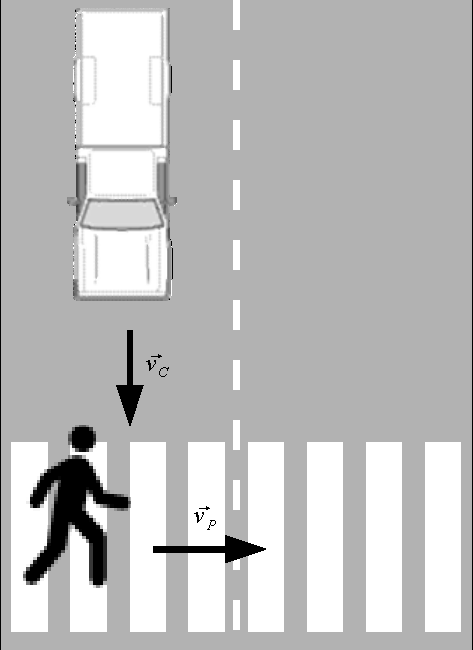
\includegraphics{img/situation.pdf}
  \caption{Overview of the situation.}
  \label{fig:situation}
\end{center}
\end{figure}

In \autoref{fig:events} the initial events in a car-pedestrian collision are
visualized. Although the pictures give the reader a good impression of what
happens during a crash, it is not entirely conforming to the situation
described above. First, in \autoref{fig:events} a normal passenger car hits the
person in front of it. The bumper of a passenger car is at a much lower height
than the bumper of a SUV. Second, there is no bull bar present.

\begin{figure}[htp]
\begin{center}
  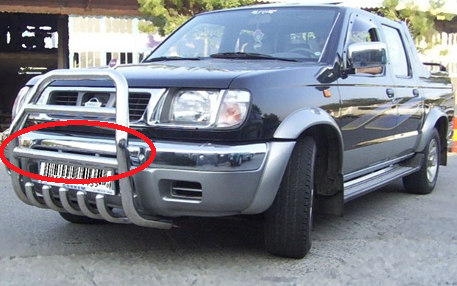
\includegraphics{img/bullbar.png}
  \caption{A bullbar mounted on a car. The protuding part is circled in red.}
  \label{fig:bullbar}
\end{center}
\end{figure}

\begin{figure}[htp]
\begin{center}
  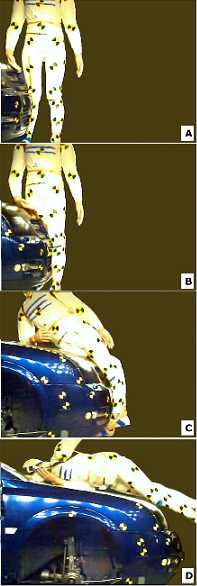
\includegraphics{img/first_instance.png}
  \caption{Subsequent events in car-pedestrian collision.}
  \label{fig:events}
\end{center}
\end{figure}

Now that the situation is properly defined, we will discuss the
assumptions we made in the next section. These will be the basis of our
mechanical analysis in \autoref{sec:analysis}